% ==============================================================================
% Section: Aggregate Bunching Diagnostic
% Status: NEW (2026-04-26 — Phase B of cap-incidence pivot)
% ==============================================================================

\section{Aggregate Bunching Diagnostic}
\label{sec:bunching}

A natural follow-on question to the cap-incidence panel of
Section~\ref{sec:cap_incidence} is whether the offer distribution itself
shows evidence of clustering near the binding administrative cap. If the
settlement cap meaningfully constrained seller bidding, one would expect
the share of resources offering at or near the cap to rise once the cap
took effect. This section reports the most direct evidence available
without unit-level offer data.

\paragraph{Data limitation.} Unit-level offer-price data for individual
generation resources are released by PJM with a roughly three-year lag,
so the 2026/27 and 2027/28 offer distributions will not be public until
2029 and 2030, respectively. The IMM does not publish a histogram of
offer prices in the State of the Market reports for any BRA. The
diagnostic in this section therefore uses the IMM-published distribution
of resources across \emph{offer-cap categories} rather than across
\emph{offer prices}. Each generation resource that submits a Capacity
Performance offer falls into one of several categories: Default ACR cap
(the resource's cost-basis offer ceiling), unit-specific calculated cap
(the IMM-computed mitigation cap above the default), uncapped planned
(Planned Generation Capacity Resources permitted to offer above the
default), or price-taker (offer at \$0, accepting clearing price). The
share of resources in each category by year is what I present.

\begin{table}[H]
  \centering
  \caption{Aggregate Offer-Cap Distribution Across Delivery Years
    (Generation Resources, RTO Level)}
  \label{tab:bunching}
  \small
  \begin{tabular}{lccccccc}
    \toprule
          & VRR    & Total      & Price  & Cost-basis & Unit-spec.\ & Uncapped & Other \\
    Year  & Design & resources  & taker  & cap        & cap          & planned  &       \\
    \midrule
    2022/23 & Old & 1,083 & 12.2\% & 80.5\% & 0.0\% & 3.2\% & 4.1\% \\
    2023/24 & Old & 1,003 & 27.0\% & 61.0\% & 7.3\% & 1.7\% & 3.0\% \\
    2024/25 & Old & 964 & 21.3\% & 74.2\% & 2.2\% & 1.8\% & 0.6\% \\
    2025/26 & Old & 1,119 & 27.1\% & 65.1\% & 5.5\% & 2.2\% & 0.1\% \\
    2026/27 & New & 1,293 & 34.8\% & 56.8\% & 6.3\% & 2.0\% & 0.0\% \\
    2027/28 & New & 1,351 & 26.9\% & 68.8\% & 1.0\% & 3.3\% & 0.0\% \\
    \bottomrule
  \end{tabular}
  \vspace{3pt}

  \begin{minipage}{0.96\textwidth}
    \footnotesize \textit{Notes:} Each cell reports the share of generation
    resources submitting Capacity Performance offers in that BRA that fall in
    the indicated offer-cap category. ``Price taker'' = offer at \$0,
    accepting clearing price. ``Cost-basis cap'' = Default ACR (or, for the
    2022/23 BRA under the old methodology, Net CONE~$\times$~B), the
    resource's cost-basis offer ceiling. ``Unit-specific cap'' = IMM-calculated
    cap above the default (APIR ACR, non-APIR ACR, standalone CPQR,
    opportunity cost, or combinations); this is the headline ``TPS mitigation''
    count of Section~\ref{sec:cap_incidence}. ``Uncapped planned'' = Planned
    Generation Capacity Resources permitted to offer above the default cost
    basis. ``Other'' includes the offer-cap option of 1.1$\times$ BRA clearing
    price (available under old methodology only) and minor combinations.
    The 2021/22 BRA (held May 2018) predates locally-available IMM SoMs and is
    omitted. Sources: IMM State of the Market Reports 2021--2025, Section~5
    Capacity, Tables 5-13/5-14/5-16/5-18 in the respective annual volumes.
  \end{minipage}
\end{table}


Table~\ref{tab:bunching} and Figure~\ref{fig:bunching} together
characterize the offer-cap composition across the six BRAs in the
sample. Two patterns are visible.

\begin{figure}[H]
  \centering
  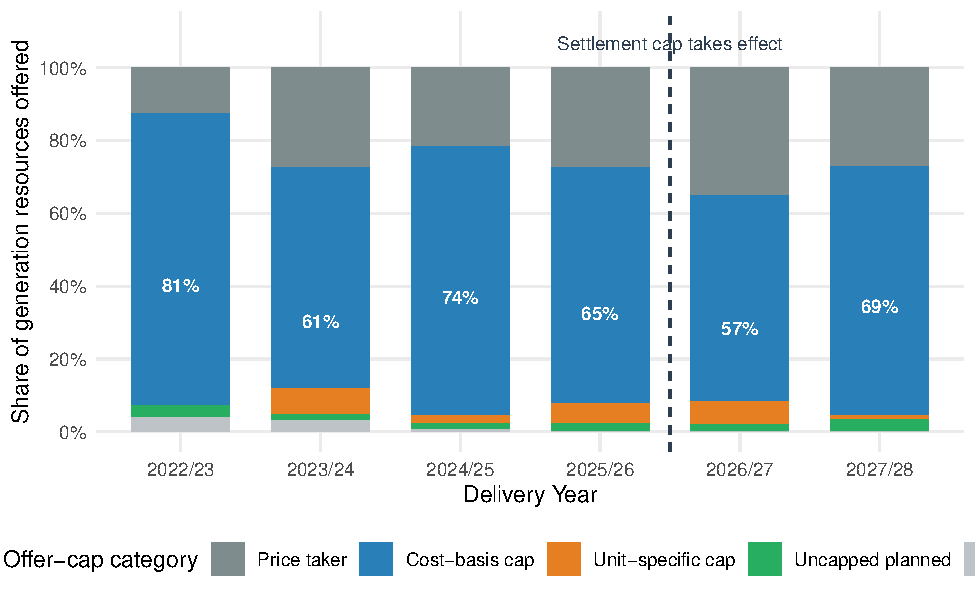
\includegraphics[width=0.95\textwidth]{../Figures/fig_bunching}
  \caption{Distribution of generation resources across offer-cap
    categories, PJM Base Residual Auctions 2022/23--2027/28 (RTO).
    The labelled percentage in each bar is the cost-basis-cap share.
    Source: IMM State of the Market Reports 2021--2025, Section~5
    Capacity, Tables 5-13/5-14/5-16/5-18 in the respective annual
    volumes.}
  \label{fig:bunching}
\end{figure}

First, the offer distribution is overwhelmingly bimodal in every year
of the sample. Resources fall into two large clusters: those offering
at \$0 as price-takers (12--35\% across years) and those offering at
their cost-basis cap (57--81\%). Together these two categories account
for 88--93\% of resources in every year. Unit-specific calculated caps
and uncapped planned generation are minor categories
(\textless10\% combined in every year). This bimodality is a structural
feature of the auction's mitigation rules, not a behavioral choice: the
Default ACR offer cap is a hard ceiling for any resource subject to
mitigation, and the price-taker option is the only alternative for
resources unwilling to compute and defend a unit-specific cap.

Second, the cost-basis-cap share does not increase systematically with
the introduction of the settlement cap. Across the six years it
fluctuates between 57\% (2026/27) and 81\% (2022/23), with no clear
trend that lines up with the cap regime. The 2027/28 BRA has the
highest cost-basis-cap share among the new-design years (68.8\%) and
the lowest unit-specific-cap share (1.0\%), consistent with the
interpretation in Section~\ref{sec:cap_incidence} that the settlement
cap moved sufficiently close to the underlying cost distribution that
fewer individual offers exceeded their unit-specific caps. But the
2026/27 cost-basis share (56.8\%) is among the lowest in the sample,
not the highest, which complicates any simple ``cap closer to clearing
$\Rightarrow$ more bunching'' narrative.

\paragraph{What this evidence does and does not show.} The aggregate
offer-cap-category data are consistent with a market structure in
which mitigation rules already produced strong bunching at unit-level
cost ceilings before the settlement, and the settlement cap then
overlay an aggregate ceiling on top of that distribution. Whether the
settlement cap induced \emph{additional} clustering near the
\$325/MW-day point (the bunching question proper) cannot be determined
from this evidence: the IMM categories aggregate across all cost-cap
levels, so a resource with an ACR of \$50/MW-day and one with an ACR
of \$300/MW-day both appear in the ``cost-basis cap'' category. The
unit-level offer histogram needed to test the bunching hypothesis
directly will not be available until 2029.

What the evidence does support is the cap-incidence framing of
Section~\ref{sec:cap_incidence}. The structural bimodality of the
offer distribution means the marginal cleared offer is, in essentially
every year, either a price-taker (when supply is loose enough that
clearing happens in the price-taker cluster) or a cost-basis-cap
offer (when supply is tight enough to push clearing into the cost-cap
cluster). In capped years, the binding administrative ceiling
truncates the upper tail of the cost-cap cluster, and clearing pins
to the cap. The dramatic price changes between regimes reflect the
clearing crossing from one cluster to the other, not changes in
seller strategy within either cluster.
